\documentclass{article}
\usepackage[utf8]{inputenc}
\usepackage[T1]{fontenc}
\usepackage[english]{babel}
\usepackage{fancyhdr}
\usepackage{svg}
\usepackage{hyperref}
\usepackage{graphicx}
\usepackage{array}
\usepackage{tabularx}
\usepackage{float}

\title{
        \vspace{-4cm}
        \begin{center}
                
\includegraphics[width=0.4\textwidth]{../asset/logo.png}
        \end{center}
        \vspace{1cm}
        {\Huge \textbf{Hypermedia Application \\ Design Report}} \\[0.5cm]
        {\large Figma: \href{https://www.figma.com/design/grXIBaO2j7GEfZ686v671W/Hyp-App?node-id=77-89&p=f&t=FRg6CJ6pKZmTnO9U-0}{https://www.figma.com/design/hypermedia2025} \\
        Website: \href{https://hmwa-25-git-main-moise7000s-projects.vercel.app}{https://hypermedia2025.vercel.app}}
}
\author{Yuto Yamaguchi \href{mailto:yuto.yamaguchi@mail.polimi.it}{yuto.yamaguchi@mail.polimi.it} \\
Xavier Anicito \href{mailto:xavierandre.anicito@mail.polimi.it}{xavierandre.anicito@mail.polimi.it} \\
Ewan Decima \href{mailto:ewangabriel.decima@mail.polimi.it}{ewangabriel.decima@mail.polimi.it}
}
\date{20 June 2025}









% Footer configuration
\pagestyle{fancy}
\fancyhf{} % clear all header and footer fields
\fancyfoot[R]{Yuto Yamaguchi, Xavier Anicito, Ewan Decima}
\renewcommand{\headrulewidth}{0pt}
\renewcommand{\footrulewidth}{0.4pt}

\begin{document}

\maketitle
\newpage
\section{Abstract}

The purpose of this design report is to provide a comprehensive overview of the key elements and decisions made
during the website implementation for a yoga center. The report meticulously outlines the primary design choices
made throughout the project, supported by relevant models, schemas, and use case scenarios. Furthermore,
it presents the conceptual and logical structure of the database, which underpins user interaction,
class scheduling, subscription management, and content delivery functionalities.
\newpage
\tableofcontents
\newpage

%\section{Abstract}

The purpose of this design report is to provide a comprehensive overview of the key elements and decisions made
during the website implementation for a yoga center. The report meticulously outlines the primary design choices
made throughout the project, supported by relevant models, schemas, and use case scenarios. Furthermore,
it presents the conceptual and logical structure of the database, which underpins user interaction,
class scheduling, subscription management, and content delivery functionalities.

\newpage


\section{Conceptual design}
This section presents an exhaustive summary of the conceptual design principles applied to the website.
It meticulously examines the decision-making process governing the content selection, its structuring into pages,
and the seamless navigation between them. The subsequent sections delve into the intricacies of these decisions,
providing a comprehensive explanation and analysis.


\subsection{C-IDM Diagram}
In this subsection, the Content Interaction Dialogue Model (C-IDM) is introduced as a model that represents the website
as a conversation between the user and the application. This model elucidates the nature of the dialogue,
including its classification, inter-relationships, and grouping of conversation topics. Additionally,
it provides insights into the content that can be discussed within each category.

\begin{figure}[h]
    \centering
    
\includegraphics[width=0.8\textwidth]{asset/c_idm_scheme}
    \caption{C-IDM Diagram}
\end{figure}


\subsection{Content-in-thesmall Tables}

\subsubsection{Topics}


\begin{center}
    \begin{tabularx}{\textwidth}{|>{\bfseries}l|X|}
        \hline
        Topic: & \textbf{Home} \\
        \hline
        Title: & text  (max 50 chars)\\
        \hline
        NewCustomerOffer: & text \\
        \hline
        FeaturedPanel: & text \\
        \hline
        DiscoverCourseLink: & URL \\
        \hline
        ContactLink: & URL \\
        \hline

    \end{tabularx}
    \caption{Table: Home}
\end{center}

\begin{center}
    \begin{tabularx}{\textwidth}{|>{\bfseries}l|X|}
        \hline
        Topic: & \textbf{Contact} \\
        \hline
        ContactInfo: & text  (max 200 chars)\\
        \hline
        ContactFormFiels: & List of text \\
        \hline
        SocialMediaLinks: & List of text \\
        \hline

    \end{tabularx}
    \caption{Table: Contact}
\end{center}


\begin{center}
    \begin{tabularx}{\textwidth}{|>{\bfseries}l|X|}
        \hline
        Topic: & \textbf{Histroy} \\
        \hline
        Title: & text  (max 200 chars)\\
        \hline
        Content: & text (max 1000 chars)\\
        \hline
        FounderImages: & List of {Image} \\
        \hline

    \end{tabularx}
    \caption{Table: History}
\end{center}


\begin{center}
    \begin{tabularx}{\textwidth}{|>{\bfseries}l|X|}
        \hline
        Topic: & \textbf{Address} \\
        \hline
        AddressText: & text  (max 200 chars)\\
        \hline
        MapEmbed: & interactive map \\
        \hline
        PublicTransportInfo: & text (max 500 chars)\\
        \hline
        OpenHoursLink: & URL \\
        \hline

    \end{tabularx}
    \caption{Table: History}
\end{center}

\begin{center}
    \begin{tabularx}{\textwidth}{|>{\bfseries}l|X|}
        \hline
        Topic: & \textbf{PracticeAtHome} \\
        \hline
        Title: & text  (max 200 chars)\\
        \hline
        Content: & text (max 500 chars) \\
        \hline
        Exercice: & text (max 500 chars)\\
        \hline
        OpenHoursLink: & URL \\
        \hline
        VideoLinks: & List of URLs \\
        \hline
        SafetyGuidelines: & text (max 500 chars) \\
        \hline


    \end{tabularx}
    \caption{Table: Practice at home}
\end{center}

\begin{center}
    \begin{tabularx}{\textwidth}{|>{\bfseries}l|X|}
        \hline
        Topic: & \textbf{OpeningHours} \\
        \hline
        WeeklySchedule: & List of {(Day, CourseName, Time)}  (max 200 chars)\\
        \hline
        PrivateCourseBookingLink: & URL \\
        \hline


    \end{tabularx}
    \caption{Table: Opening Hours}
\end{center}

\begin{center}
    \begin{tabularx}{\textwidth}{|>{\bfseries}l|X|}
        \hline
        Topic: & \textbf{Benefit} \\
        \hline
        Title: & text  (max 200 chars)\\
        \hline
        Content: & text (max 500 chars) \\
        \hline
        FeatureList: & List of {(Benefit, Description)} (max 500 chars)\\
        \hline
        RelatedLink: & URL \\
        \hline

    \end{tabularx}
    \caption{Table: Benefit}
\end{center}


\begin{center}
    \begin{tabularx}{\textwidth}{|>{\bfseries}l|X|}
        \hline
        Topic: & \textbf{Equipement} \\
        \hline
        Title: & text  (max 200 chars)\\
        \hline
        Content: & text (max 500 chars) \\
        \hline
        FeatureList: & List of {(Benefit, Description)} (max 500 chars)\\
        \hline
        RelatedLink: & URL \\
        \hline

    \end{tabularx}
    \caption{Table: Equipement}
\end{center}

\subsubsection{Kind of Topic}

\begin{center}
    \begin{tabularx}{\textwidth}{|>{\bfseries}l|X|}
        \hline
        Kind of topic: & \textbf{Course} \\
        \hline
        Title: & text  (max 200 chars)\\
        \hline
        Image: & image \\
        \hline
        Description: & text (max 500 chars) \\
        \hline
        Goal: & text (max 200 chars) \\
        \hline
        Timetable: & List of {(Day, Time)}\\
        \hline
        Price: & currency \\
        \hline
        IntroVideoUrl: & URL \\
        \hline
        TaughtBy: & List of {Teachers, Link} \\
        \hline
        PartOfSubscription: & List of {(Subscription, Link)} \\
        \hline
        CoveredInArticle: & List of {(Article, Link)}\\
        \hline
    \end{tabularx}
    \caption{Table: Course}
\end{center}

\begin{center}
    \begin{tabularx}{\textwidth}{|>{\bfseries}l|X|}
        \hline
        Kind of Topic: & \textbf{Subscription} \\
        \hline
        Name: & text  (max 200 chars)\\
        \hline
        Type: & text (max 200 chars) \\
        \hline
        TotalCourse: & integer \\
        \hline
        Price: & Currency \\
        \hline
        Link: & URL \\
        \hline
        ContactLink: & URL \\
        \hline
        Details: & text (max 500 chars) \\
        \hline
        CoursesIncluded: & List of {(CourseTitle, Link)}\\
        \hline
    \end{tabularx}
    \caption{Table: Equipement}
\end{center}

\begin{center}
    \begin{tabularx}{\textwidth}{|>{\bfseries}l|X|}
        \hline
        Kind of Topic: & \textbf{Event} \\
        \hline
        Title: & text  (max 200 chars)\\
        \hline
        Image: & Image \\
        \hline
        Date: Timestamp \\
        \hline
        Description: & text (max 500 chars) \\
        \hline
        Location: & text (max 500 chars) \\
        \hline
        BookingLink: & URL \\
        \hline
        HostedBy: & List of {(Teachers, Link)} \\
        \hline
        CoveredInArticles: List of {(Article, Link)}\\
        \hline

    \end{tabularx}
    \caption{Table: Event}
\end{center}

\begin{center}
    \begin{tabularx}{\textwidth}{|>{\bfseries}l|X|}
        \hline
        Kind of Topic: & \textbf{Teacher} \\
        \hline
        Name: & text  (max 200 chars)\\
        \hline
        Photo: & Image \\
        \hline
        Biography: & text (max 500 chars) \\
        \hline
        Certificates: & List of {Image or Text} \\
        \hline
        CoursesTaught: & List of {(Course, Link)} \\
        \hline
        SocialMedias: & List of {URL} \\
        \hline
        HostedEvents: & List of {(Event, Link)}
        \hline
        AuthoredArticles: & List of {(Article, Link)} \\
        \hline

    \end{tabularx}
    \caption{Table: Teacher}
\end{center}
\begin{center}
    \begin{tabularx}{\textwidth}{|>{\bfseries}l|X|}
        \hline
        Kind of Topic: & \textbf{Article} \\
        \hline
        Title: & text  (max 200 chars)\\
        \hline
        ThumbnailImage: & Image \\
        \hline
        Snippet: & text (max 200 chars) \\
        \hline
        FullText: & text \\
        \hline
        Authors: & List of {Text or (Teachers, Link)}
        \hline
        PublishDate: & Date (Timestamp) \\
        \hline
        AboutCourses: & List of {Course, Link} \\
        \hline
        AboutEvents: & List of {(Event, Link)}
        \hline
    \end{tabularx}
    \caption{Table: Article}
\end{center}

\subsubsection{Group of Topics}
\begin{center}
    \begin{tabularx}{\textwidth}{|>{\bfseries}l|X|}
        \hline
        Group: & \textbf{AllCourses} \\
        \hline
        Title: & text  (max 200 chars)\\
        \hline
        Description: & text (max 500 chars) \\
        \hline
        MembersPreview: & List of {(Course, Thumbnail, Title, Price)} \\
        \hline

    \end{tabularx}
    \caption{Table: All Courses }
\end{center}

\begin{center}
    \begin{tabularx}{\textwidth}{|>{\bfseries}l|X|}
        \hline
        Group: & \textbf{AllSubscription} \\
        \hline
        Title: & text  (max 200 chars)\\
        \hline
        Description: & text (max 500 chars) \\
        \hline
        MembersPreview: & List of {(Subscription, Name, TotalCourses, Price)} \\
        \hline

    \end{tabularx}
    \caption{Table: All Subscriptions }
\end{center}

\begin{center}
    \begin{tabularx}{\textwidth}{|>{\bfseries}l|X|}
        \hline
        Group: & \textbf{AllEvents} \\
        \hline
        Title: & text  (max 200 chars)\\
        \hline
        Description: & text (max 500 chars) \\
        \hline
        MembersPreview: & List of {(Event, Thumbnail, Title, Date)} \\
        \hline

    \end{tabularx}
    \caption{Table: All Events }
\end{center}

\begin{center}
    \begin{tabularx}{\textwidth}{|>{\bfseries}l|X|}
        \hline
        Group: & \textbf{AllTeachers} \\
        \hline
        Title: & text  (max 200 chars)\\
        \hline
        Description: & text (max 500 chars) \\
        \hline
        MembersPreview: & List of {(Teacher, Names, CoursesTaught)} \\
        \hline

    \end{tabularx}
    \caption{Table: All Teachers }
\end{center}

\begin{center}
    \begin{tabularx}{\textwidth}{|>{\bfseries}l|X|}
        \hline
        Group: & \textbf{InstitueSection} \\
        \hline
        Title: & text  (max 200 chars)\\
        \hline
        Description: & text (max 500 chars) \\
        \hline
        MembersPreview: & List of {(SectionTitle, Snippet)} \\
        \hline

    \end{tabularx}
\end{center}


\begin{center}
    \begin{tabularx}{\textwidth}{|>{\bfseries}l|X|}
        \hline
        Group: & \textbf{AboutYogaTopics} \\
        \hline
        Title: & text  (max 200 chars)\\
        \hline
        Description: & text (max 500 chars) \\
        \hline
        MembersPreview: & List of {(TopicTitle, Link)} \\
        \hline

    \end{tabularx}
    \caption{Table: About Yoga Topics }
\end{center}

\begin{center}
    \begin{tabularx}{\textwidth}{|>{\bfseries}l|X|}
        \hline
        Group: & \textbf{AllYogaArticles} \\
        \hline
        Title: & text  (max 200 chars)\\
        \hline
        Description: & text (max 500 chars) \\
        \hline
        MembersPreview: & List of {(Article, Thumbnail, Title, PublishDate)} \\
        \hline

    \end{tabularx}
    \caption{Table: All Yoga Articles}
\end{center}

\section{Final Commented Screenshots}

\subsection{Topic}

\paragraph{Home} \mbox{}\\
The website’s home page serves as an inviting gateway to the yoga center’s digital presence. As the initial interaction
users have with the organization, it was meticulously designed to provide a comprehensive and user-friendly overview of
the studio’s offerings. Through strategically placed navigation links, promotional banners, and well-structured
sections, the page seamlessly guides users through exploring classes, subscriptions, equipment, and wellness
resources available across the website.

\begin{figure}[H]
    \centering
    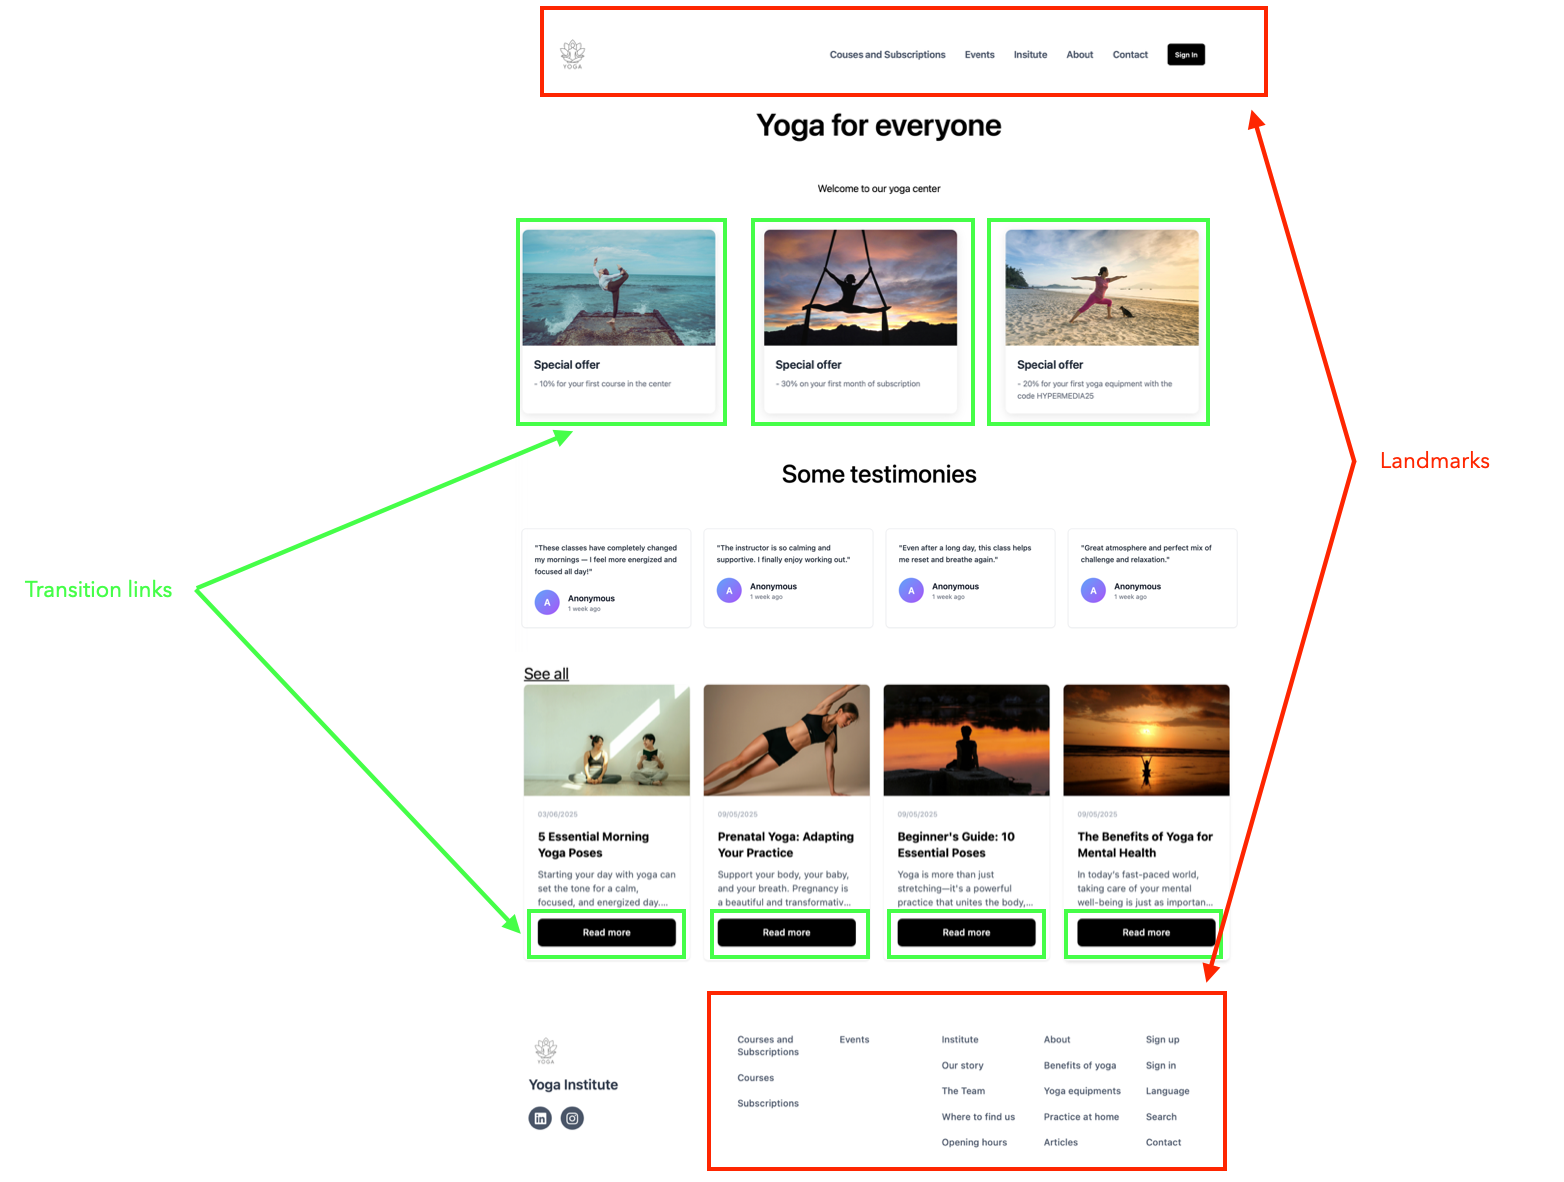
\includegraphics[width=0.8\textwidth]{asset/screen/homepage}
    \caption{Home Page}
\end{figure}

\subsection{Single Topic Pages}




\paragraph{Contact us Page} \mbox{}\\


The primary objective of this page is to facilitate communication between users seeking information about the center
or yoga in general. Frequently asked questions are prominently displayed, accompanied by a comprehensive and clearly
outlined form for users to complete.

\mbox{}\\

\begin{figure}[H]
    \centering
    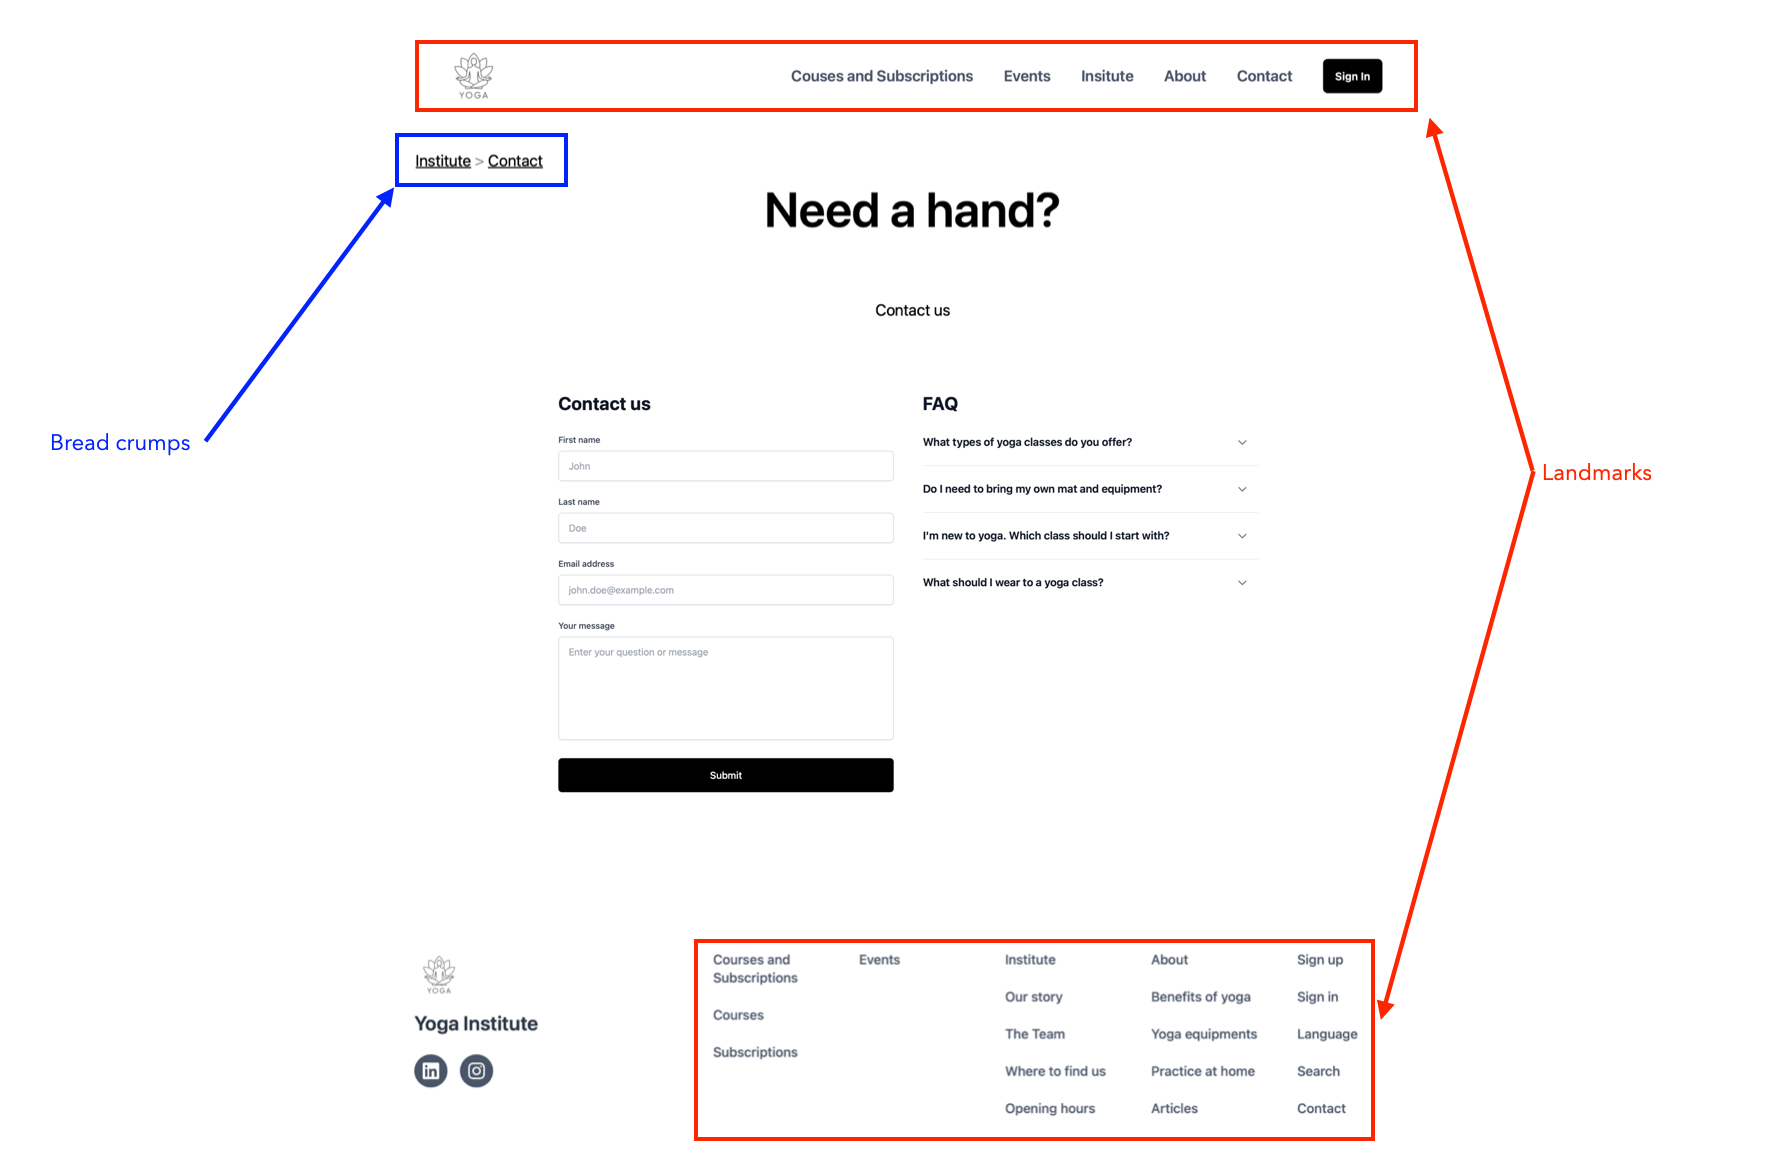
\includegraphics[width=1\textwidth]{asset/screen/contact_us}
    \caption{Contact us Page}
\end{figure}

\subsection{Group Page}


\paragraph{All Courses} \mbox{}\\
The \textit{All Courses} page provides users with a clear and organized overview of all yoga classes offered by the studio.
Designed with accessibility and clarity in mind, this section allows visitors to easily browse through the
variety of courses available, each tailored to different skill levels.

\begin{figure}[H]
    \centering
    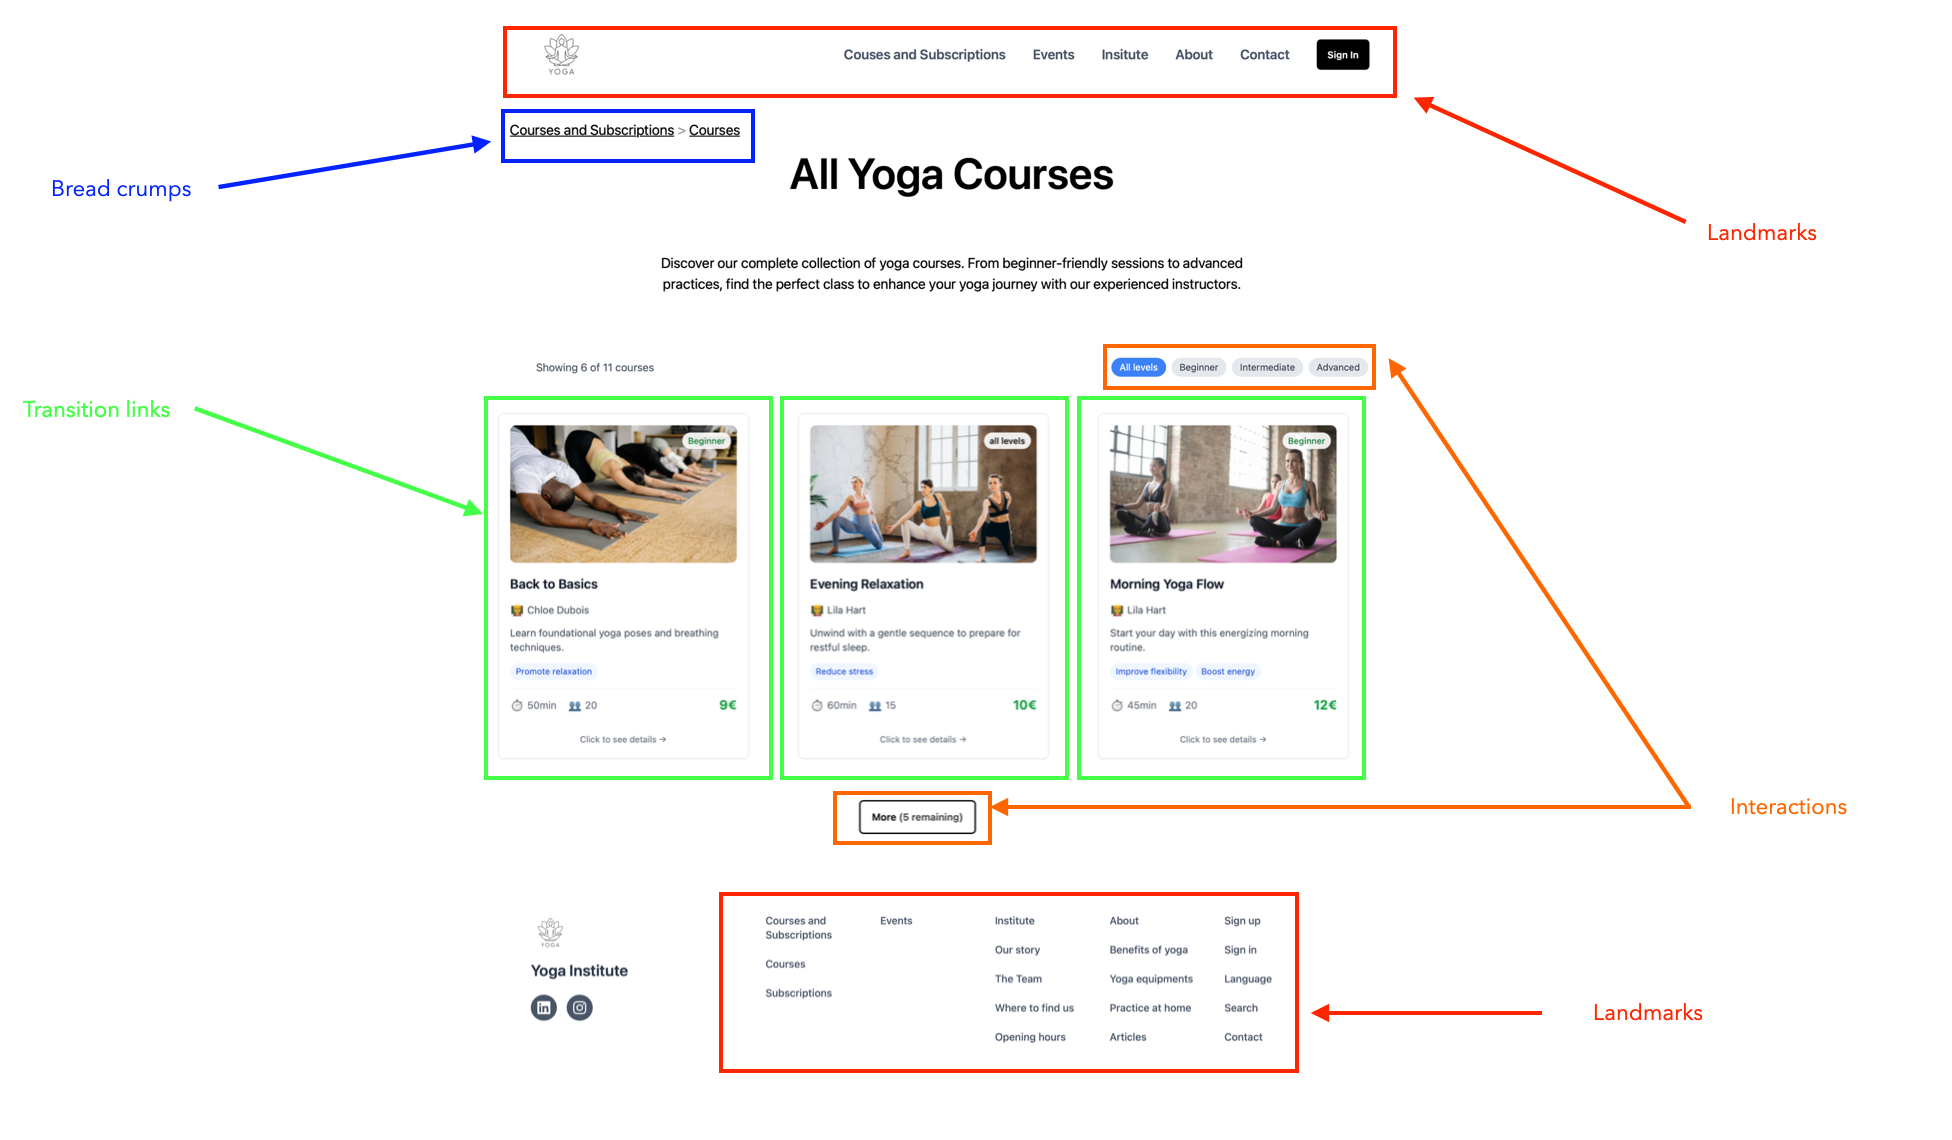
\includegraphics[width=0.8\textwidth]{asset/screen/courses}
    \caption{All Courses Page}
\end{figure}

\subsection{Kind Topic Pages}


\paragraph{All Courses} \mbox{}\\
The \textit{Course} page provides information about one yoga class taught at the institute.

\mbox{}\\

\begin{figure}[H]
    \centering
    
\includegraphics[width=1\textwidth]{asset/screen/course}
    \caption{A course page}
\end{figure}



\usepackage{tabularx}
\usepackage{caption}

\newcommand{\usecasetable}[6]{%
    \begin{center}
    \begin{tabularx}{\textwidth}{|>{\bfseries}l|X|}
    \hline
    Title: & #1 \\
    \hline
    Profile: & #2 \\
    \hline
    Goal: & #3 \\
    \hline
    Context: & #4 \\
    \hline
    Tasks: & #5 \\
    \hline
    \end{tabularx}
    \end{center}
}

\section{Interaction scenarios}

This section presents concrete examples demonstrating how users will interact with the web application. It meticulously
outlines the sequence of actions necessary to access the site’s content and features. Each interaction scenario
embodies a realistic use case and is accompanied by a descriptive narrative and visual aids, with interactive elements
explicitly highlighted.

\subsection{Use case 1}
\subsubsection{Textual narrative}


\usecasetable
    {Find how to reach the center in metroline}
    {A potential customer seeking to access the yoga center via the metro system}
    {Their goal is to find the metro route from their current location to the yoga center}
    {They access the web application from any personal device}
    {\begin{itemize}
         \item They access the \textit{Home page} of the website
         \item They navigate to the \textit{Institute} page using the navigation bar. Then, they click on the
               \textit{Where to find us?} button, which leads them to the \textit{Location} page, where an interactive map displays the center’s address. Alternatively, they can access the \textit{Location} page directly via the navigation bar.
    \end{itemize}
    }


\subsubsection{Interaction Flow}

\begin{figure}[H]
    \centering
    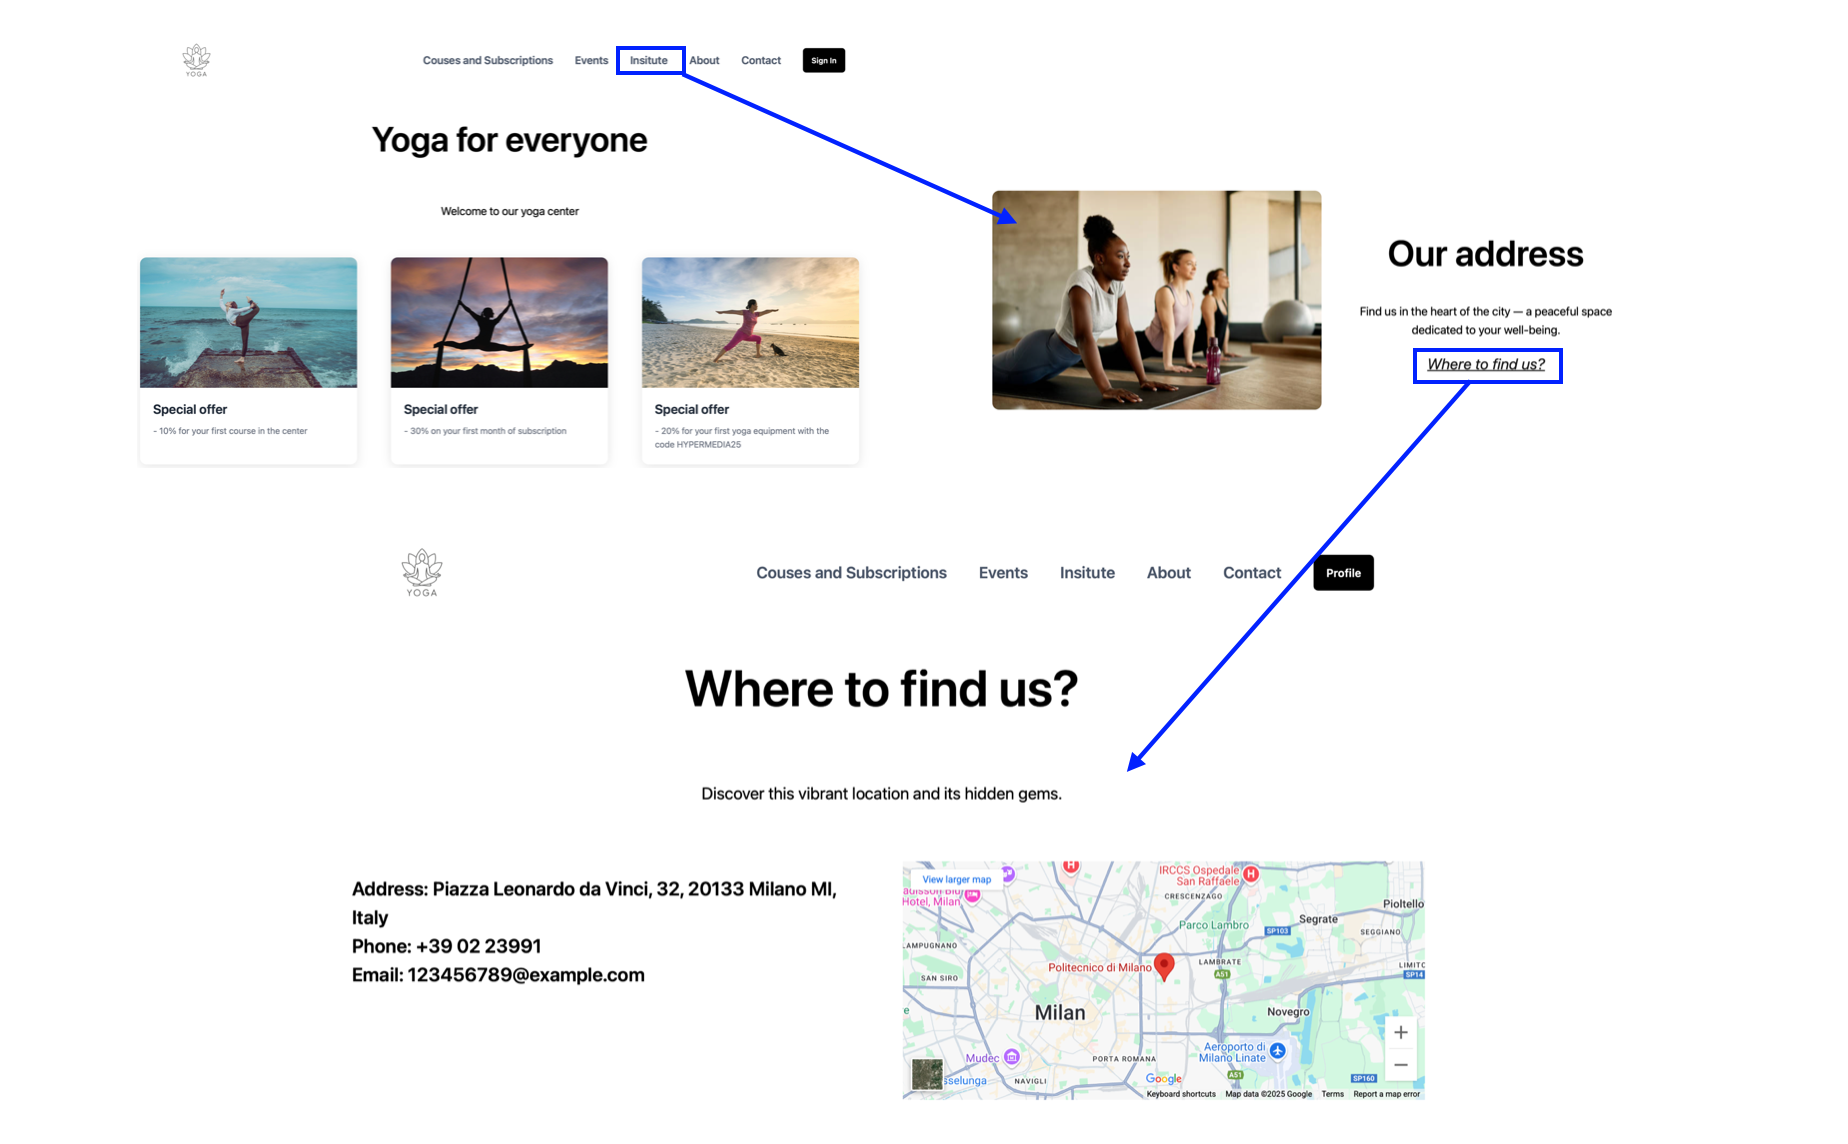
\includegraphics[width=0.9\textwidth]{asset/interactive_flow/location}
    \caption{Use case 1: Find the location of the center}
\end{figure}


\subsection{Use case 2}
\subsubsection{Textual narrative}

\usecasetable
    {Find somewhere to contact the center}
    {A potential customer seeking to reach the yoga center}
    {Their goal is to find a way to contact the center}
    {They access the web application from any personal device}
    {\begin{itemize}
         \item They access the \textit{Home page} of the website
         \item They navigate to the \textit{Contact} page using the navigation bar.
         \item They have the capability to compose messages via the contact form.
    \end{itemize}
    }


\subsubsection{Interaction Flow}
\begin{figure}[H]
    \centering
    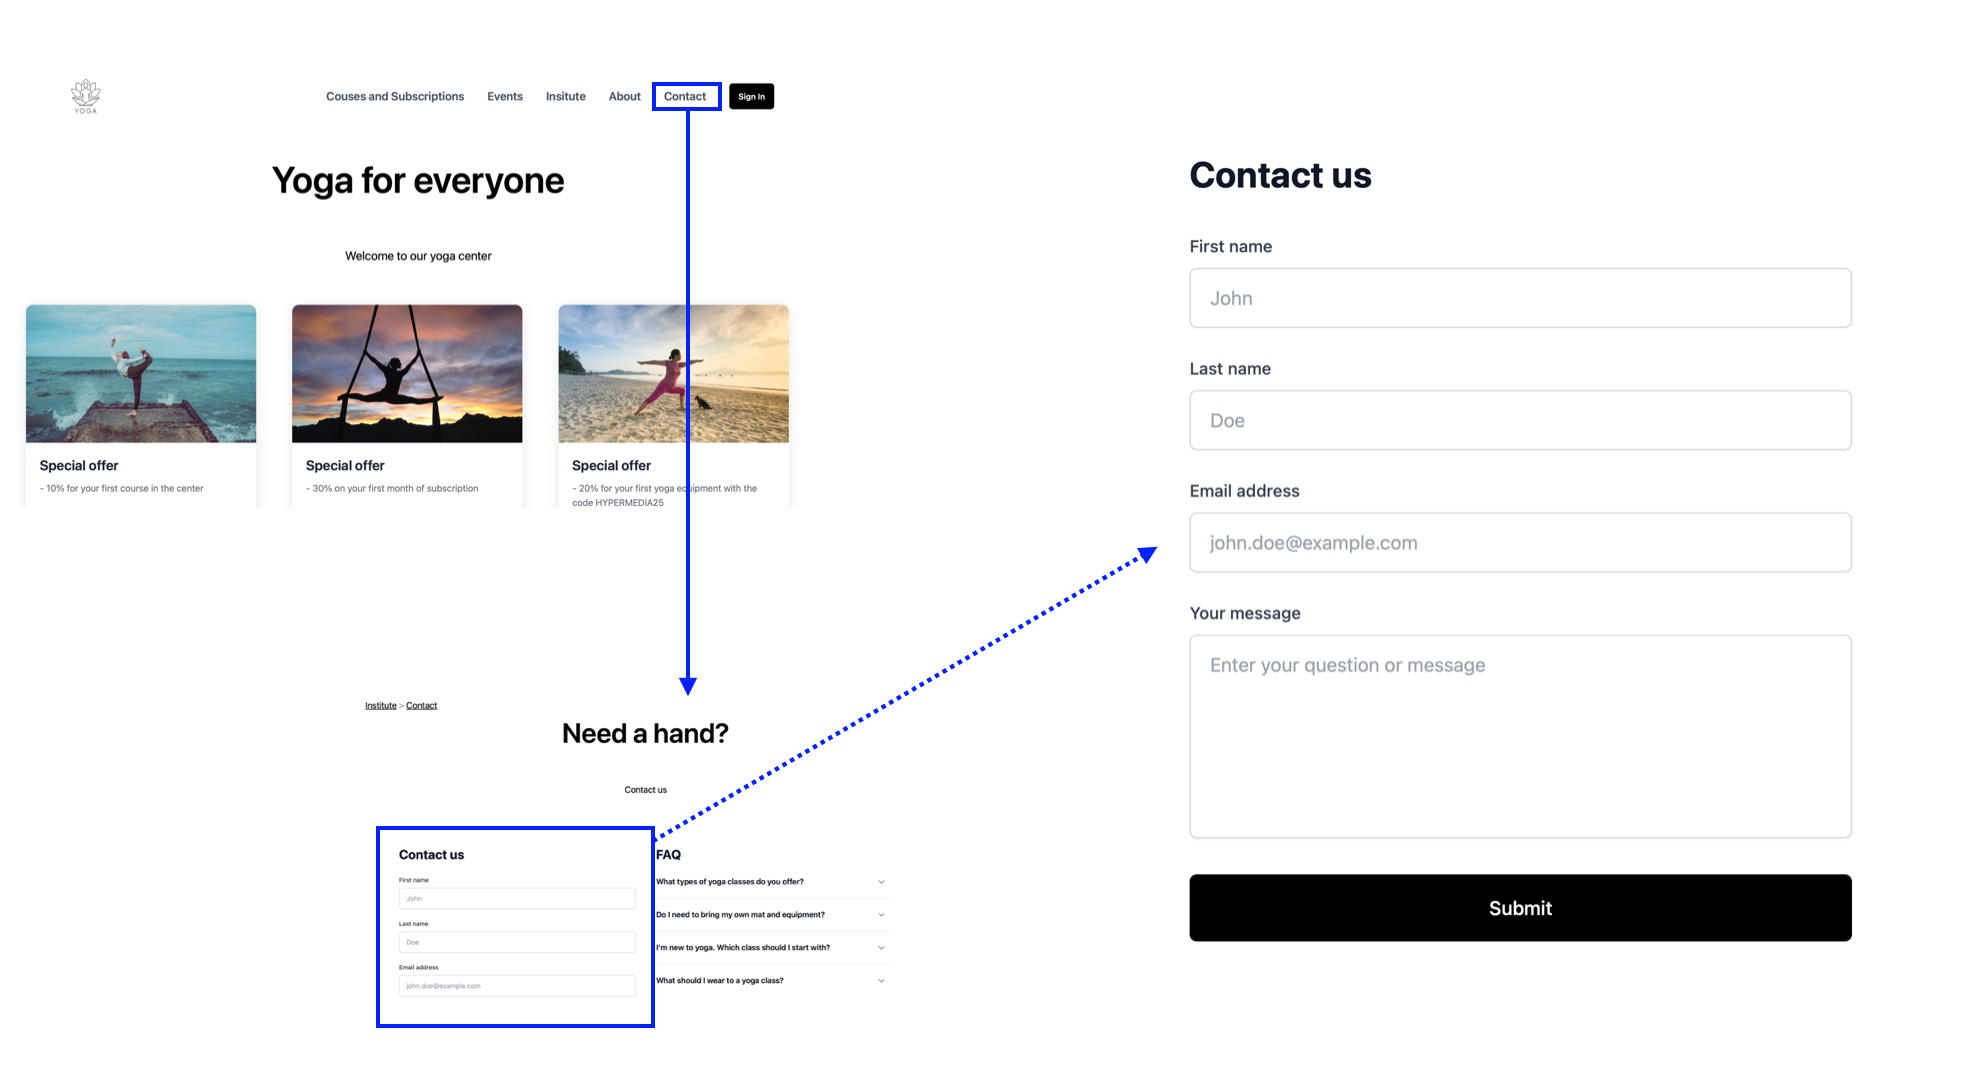
\includegraphics[width=0.9\textwidth]{asset/interactive_flow/contact}
    \caption{Use case 2: Find a way to contact the center}
\end{figure}


\subsection{Use case 3}
\subsubsection{Textual narrative}
\usecasetable
    {You want to know some exercices you can do at home}
    {A user seeking to practice at home}
    {Their goal is to find exercices and instructions to practice yoga at home}
    {They access the web application from any personal device}
    {\begin{itemize}
         \item They access the \textit{Home page} of the website
         \item They navigate to the \textit{About} page using the navigation bar. Then, they click on the
         \textit{Start now} button, which leads them to the \textit{Practice at home} page, where they can find a list of exercices, tutorials videos and some guidelines. Alternatively, they can access the \textit{Practice at home} page directly via the navigation bar.
    \end{itemize}
    }

\subsubsection{Interaction Flow}
\begin{figure}[H]
    \centering
    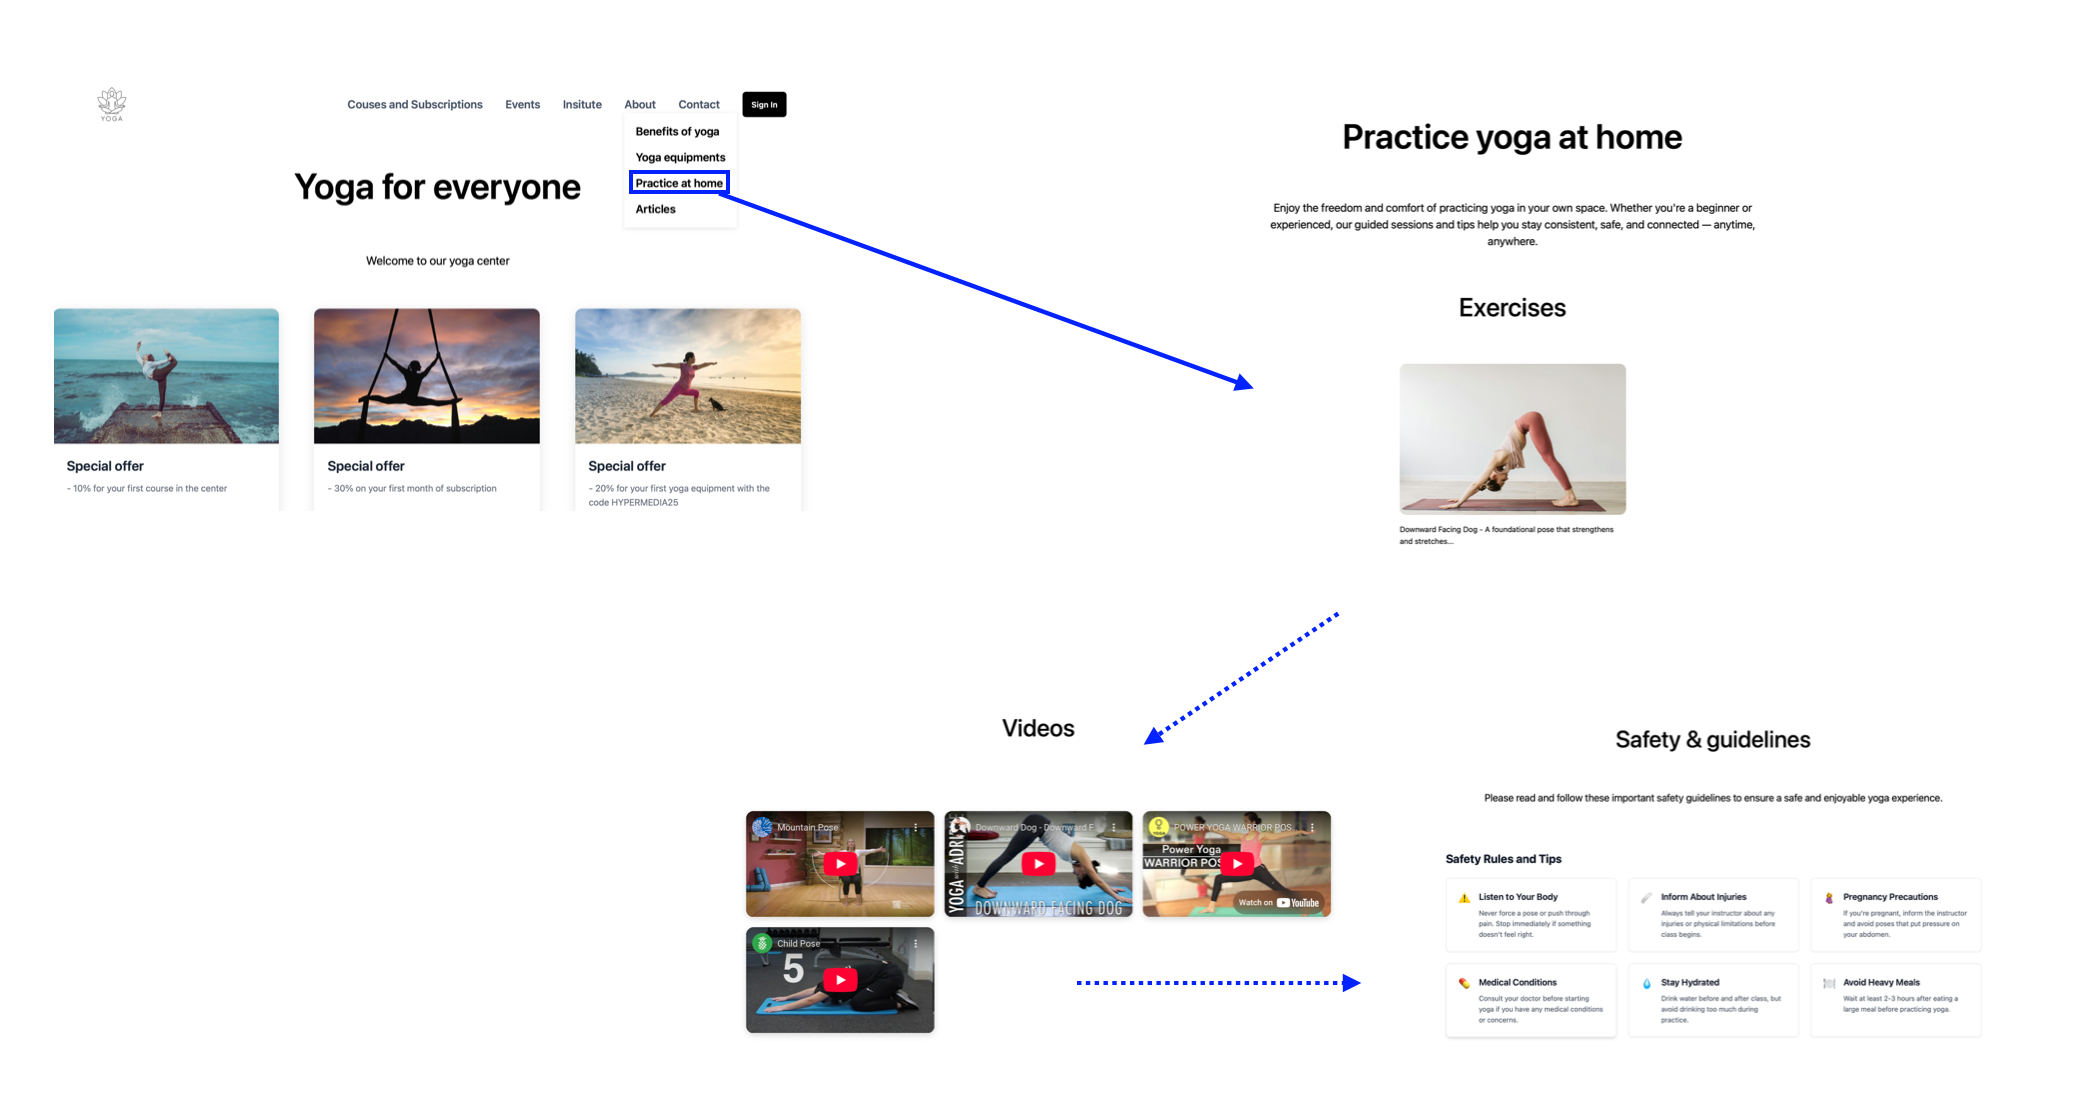
\includegraphics[width=0.9\textwidth]{asset/interactive_flow/practice}
    \caption{Use case 3: Find a way to practice yoga at home}
\end{figure}

\subsection{Use case 4}
\subsubsection{Textual narrative}
\usecasetable
    {Your friend recommanded you their favorite teacher, \textit{Chloe Dubois}, and you want to try some courses with her. Find her courses and then find the conditions to participate at 3 courses of her at the best price.}
    {A new visitor who heard about the yoga center through a friend. They are curious and motivated to try classes with a specific teacher and want to explore flexible options to attend three of her sessions at the best price.}
    {Their goal is to find the most affordable way to enroll in Chloe Dubois’s courses}
    {They access the web application from any personal devicer}
    {\begin{itemize}
         \item They access the \textit{Home page} of the website
         \item They navigate to the \textit{Institute} page using the navigation bar. Then, they click on the
                \textit{See your teachers} button, which leads them to the \textit{Teachers} page, where they can find all the
                center's teachers. Alternatively, they can access the \textit{Teachers} page directly via the navigation bar by clicking the \textit{The team} button.
         \item They click on \textit{Chloe Dubois' card} in order to see her profile and all her courses
         \item The can click on any \textit{course card} to see price and description
    \end{itemize}
    }

\subsubsection{Interaction Flow}




%You are looking for something to do on Tuesday afternoon, find which courses are given
%You are looking for an event on next Hollydays, find which event takes place between June 7th and June 12th


\newpage

\section{Database Design}

This section presents the design of the database for the website to be implemented. Indeed, it manages students, teachers, courses, subscriptions, feedback,
equipment, events, and articles. The schema includes detailed relationships between entities, such as students
enrolling in courses, courses requiring specific equipment, and subscriptions granting access to various learning materials. JSON fields are used for flexible
data such as certificates, goals, and social media links.



\subsection{Explanation of Relationship Symbols}

The following notation is used in the Entity-Relationship (ER) diagrams, following the Mermaid syntax conventions that
you can check on : \href{https://mermaid.js.org/syntax/entityRelationshipDiagram.html}{mermaid.js.org}

\subsection{Entity-Relation Diagram}

\begin{figure}[H]
    \centering
    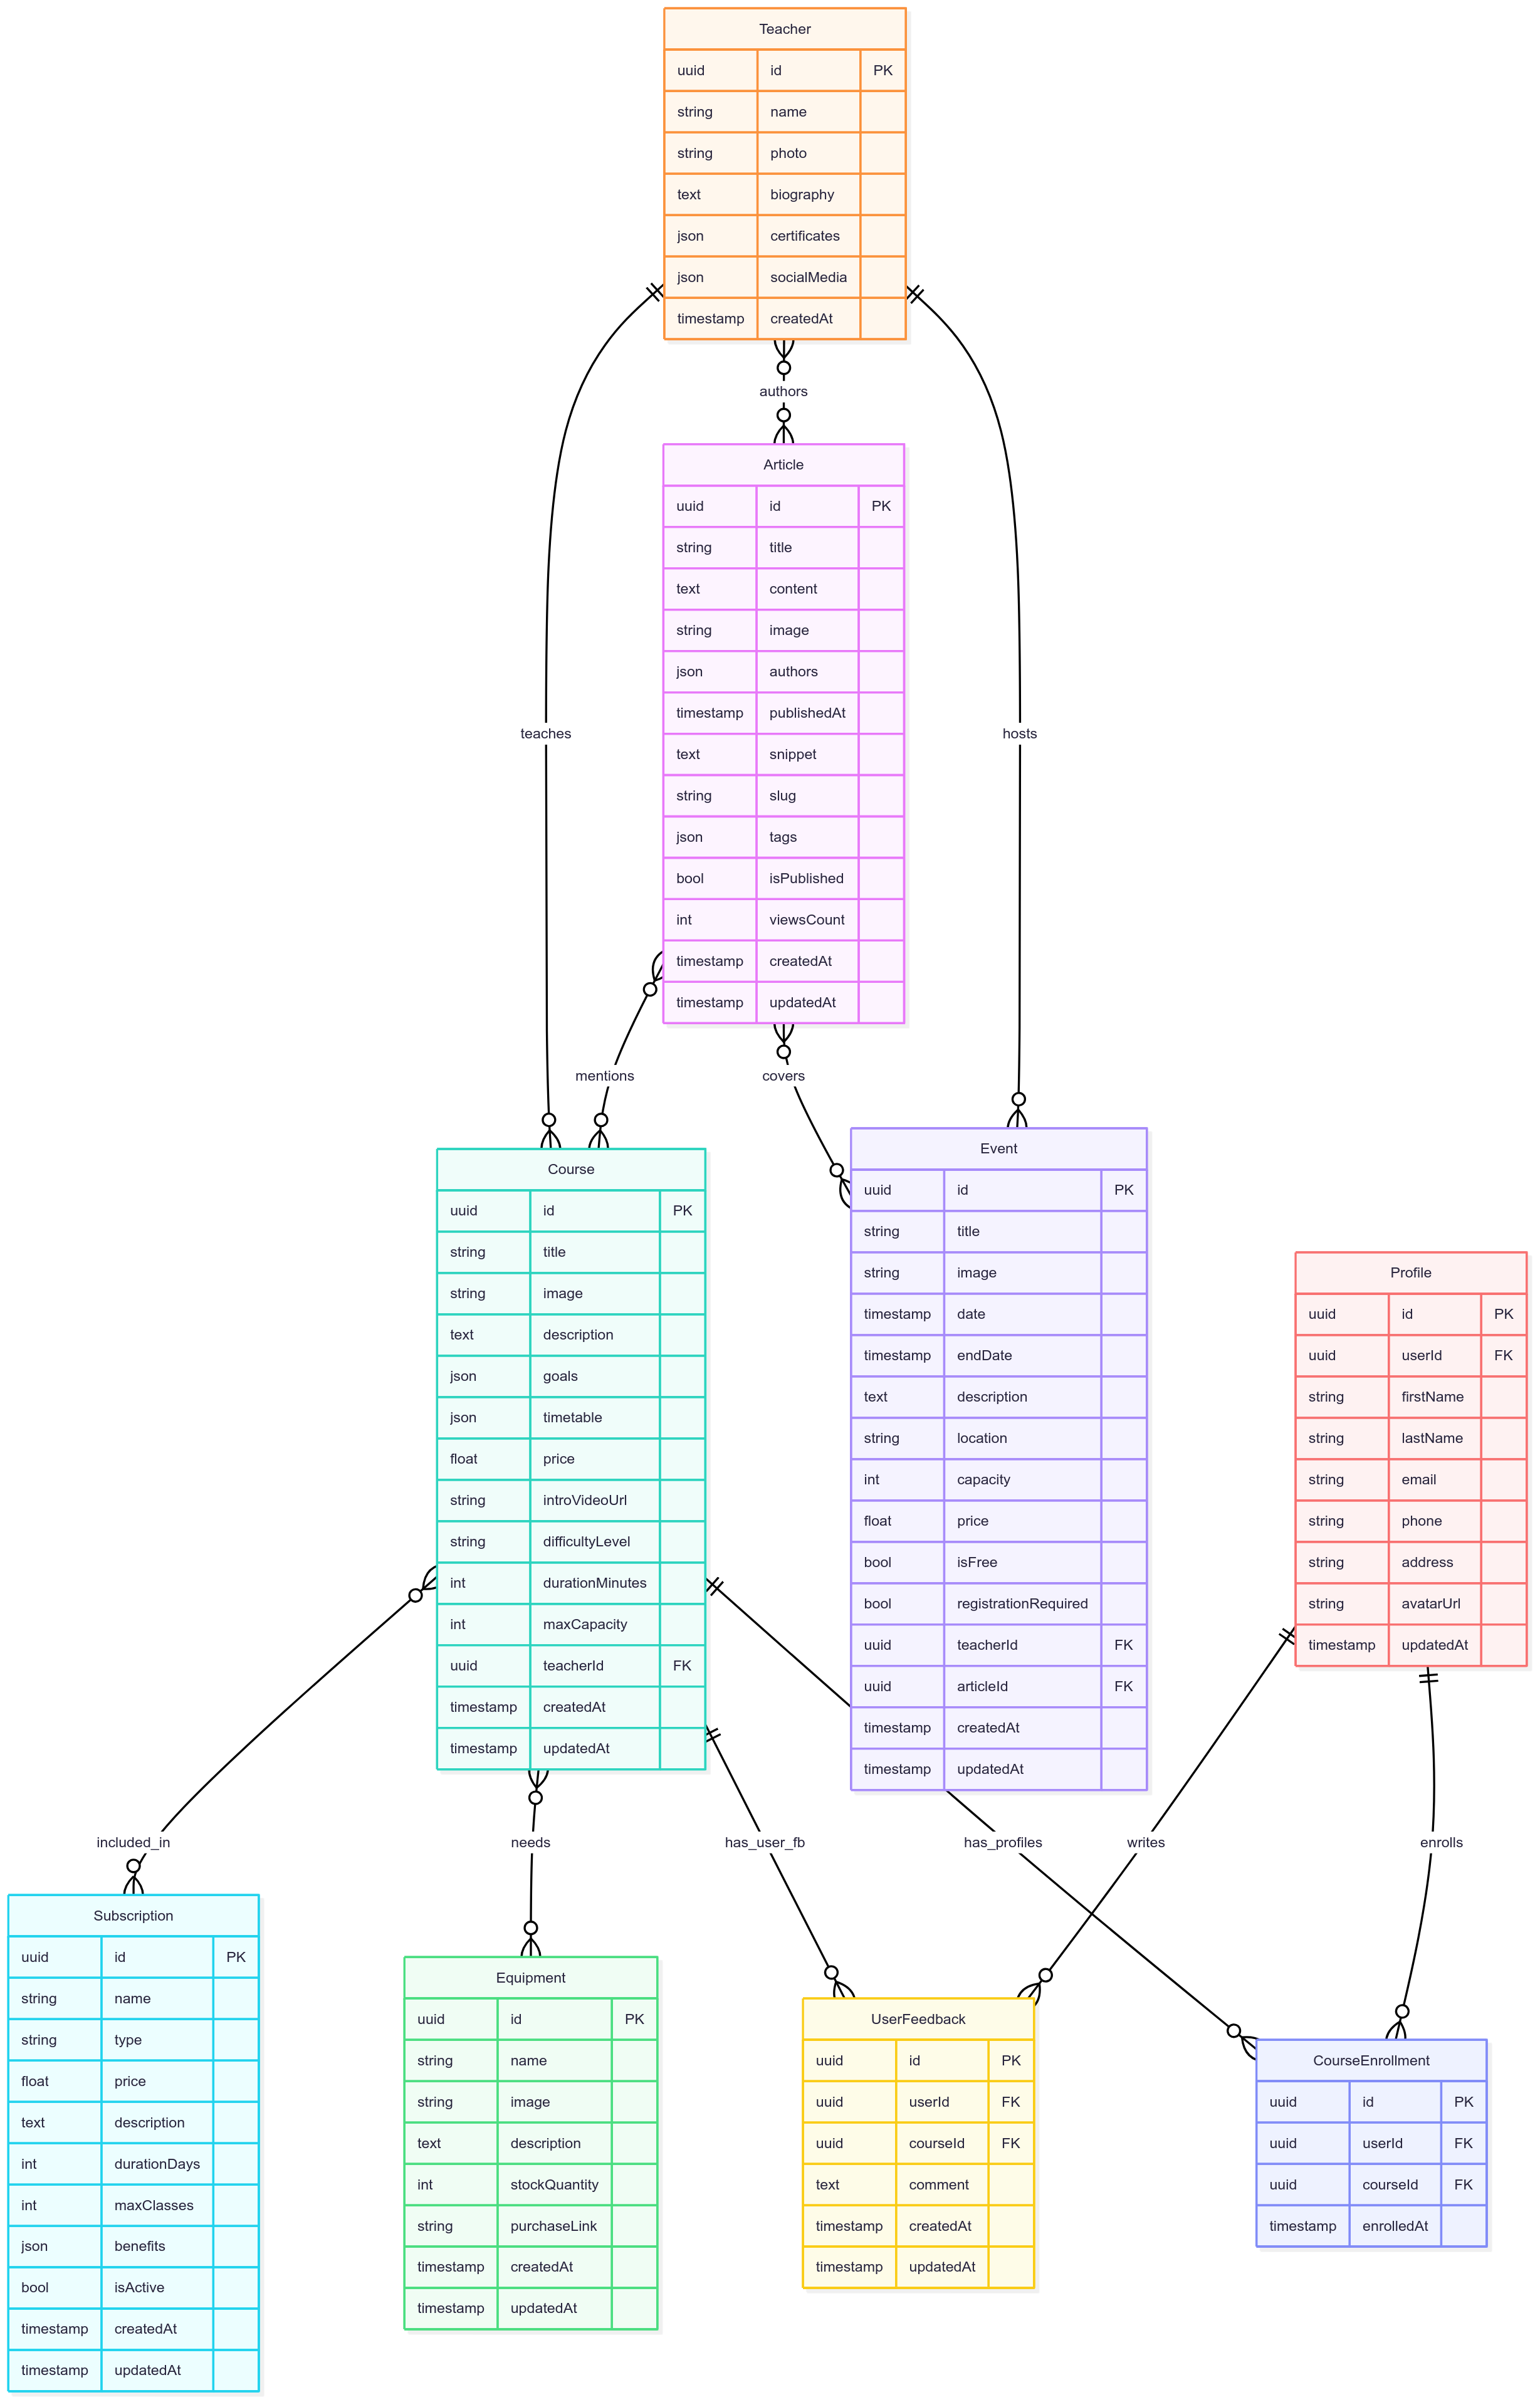
\includegraphics[width=0.6\textwidth]{asset/new_database_e_r_diagram.png}
    \caption{E-R Diagram}
\end{figure}

\newpage
\section{Annex}

\subsection{Division of the work}

In the design phase, all members contributed to do the CIDM diagram, the abstract tables and pages and the wireframes. The group divided the work for the Figma design.

In the technological phase, Ewan did the database and the data-related scripts and all the members contributed to the implementation of the Nuxt components.

Xavier focused on the textual narrative of the use cases, Yuto prepared the pictures for the report and all members contributed to its writing.

\subsection{Abstract pages}

\subsubsection{Topics}

\begin{table}[H]
\centering
\begin{tabularx}{\textwidth}{|>{\bfseries}l|X|}
\hline
Topic: & \textbf{Home} \\
\hline
Title & Text (max 20 chars) e.g., "Welcome to Yoga Website" \\
\hline
NewCustomerOffer & List of (Image, Title, Description) \\
\hline
Testimonies & List of (Text, Image, Name, Time) \\
\hline
RelatedArticles & List of (Image, Date, Title, Description, Button) \\
\hline
Landmarks & Navigation bars \\
\hline
Breadcrumbs & — \\
\hline
\end{tabularx}
\caption{Table: Home}
\end{table}

\begin{table}[H]
\centering
\begin{tabularx}{\textwidth}{|>{\bfseries}l|X|}
\hline
Topic: & \textbf{Contact} \\
\hline
Title & Text (max 30 chars) \\
\hline
Subtitle & Text (max 150 chars) \\
\hline
ContactFormFields & List of (Name, Email, Message) \\
\hline
FAQ & List of (Question, Answer) \\
\hline
Landmarks & Navigation bars \\
\hline
Breadcrumbs & — \\
\hline
\end{tabularx}
\caption{Table: Contact}
\end{table}

\begin{table}[H]
\centering
\begin{tabularx}{\textwidth}{|>{\bfseries}l|X|}
\hline
Topic: & \textbf{OurStory} \\
\hline
Title & Text (max 30 chars) \\
\hline
Subtitle & Text (max 150 chars) \\
\hline
MainImage & Image \\
\hline
Topics & List of (Image, Title, Description) \\
\hline
Landmarks & Navigation bars \\
\hline
Breadcrumbs & — \\
\hline
\end{tabularx}
\caption{Table: Our Story}
\end{table}

\begin{table}[H]
\centering
\begin{tabularx}{\textwidth}{|>{\bfseries}l|X|}
\hline
Topic: & \textbf{WhereToFindUs} \\
\hline
Title & Text (max 30 chars) \\
\hline
Description & Text (max 150 chars) \\
\hline
AddressText & Text (max 200 chars) \\
\hline
MapEmbed & Interactive map widget \\
\hline
Access & Text (max 500 chars) \\
\hline
Insights & Text (max 500 chars) \\
\hline
NerbyAmenities & Text (max 500 chars) \\
\hline
Landmarks & Navigation bars \\
\hline
Breadcrumbs & — \\
\hline
\end{tabularx}
\caption{Table: Where To Find Us}
\end{table}

\begin{table}[H]
\centering
\begin{tabularx}{\textwidth}{|>{\bfseries}l|X|}
\hline
Topic: & \textbf{PracticeAtHome} \\
\hline
Title & Text (max 30 chars) \\
\hline
Description & Text (max 150 chars) \\
\hline
ExerciseList & List of (Image, Instruction) \\
\hline
VideoLinks & List of URLs \\
\hline
SafetyGuidelines & List of Rules \\
\hline
Landmarks & Navigation bars \\
\hline
Breadcrumbs & — \\
\hline
\end{tabularx}
\caption{Table: Practice at Home}
\end{table}

\begin{table}[H]
\centering
\begin{tabularx}{\textwidth}{|>{\bfseries}l|X|}
\hline
Topic: & \textbf{Equipment} \\
\hline
Title & Text (max 30 chars) e.g., "Yoga Equipment" \\
\hline
Description & Text (max 150 chars) – Introduction to mats, blocks, straps \\
\hline
EquipmentList & List of (Name, Image, Description, Link) \\
\hline
Landmarks & Navigation bars \\
\hline
Breadcrumbs & — \\
\hline
\end{tabularx}
\caption{Table: Equipment}
\end{table}

\begin{table}[H]
\centering
\begin{tabularx}{\textwidth}{|>{\bfseries}l|X|}
\hline
Topic: & \textbf{OpeningHours} \\
\hline
Title & Text (max 30 chars) \\
\hline
Description & Text (max 150 chars) \\
\hline
Timetable & List of (Day, Course, Time) \\
\hline
Landmarks & Navigation bars \\
\hline
Breadcrumbs & — \\
\hline
\end{tabularx}
\caption{Table: Opening Hours}
\end{table}

\subsubsection{Kinds of topics}

\begin{table}[H]
\centering
\begin{tabularx}{\textwidth}{|>{\bfseries}l|X|}
\hline
Kind of Topic: & \textbf{Course} \\
\hline
Title & Text (max 200 chars) \\
\hline
Image & Image \\
\hline
Description & Text (max 500 chars) \\
\hline
Goal & Text (max 200 chars) \\
\hline
Timetable & List of (Day, Time) \\
\hline
Price & Currency \\
\hline
IntroVideoUrl & URL \\
\hline
TaughtBy & List of (Teacher, Link) \\
\hline
PartOfSubscription & List of (Subscription, Link) \\
\hline
CoveredInArticle & List of (Article, Link) \\
\hline
\end{tabularx}
\caption{Table: Course}
\end{table}

\begin{table}[H]
\centering
\begin{tabularx}{\textwidth}{|>{\bfseries}l|X|}
\hline
Kind of Topic: & \textbf{Subscription} \\
\hline
Name & Text (max 200 chars) \\
\hline
Type & Text (max 200 chars) \\
\hline
TotalCourse & Integer \\
\hline
Price & Currency \\
\hline
Link & URL \\
\hline
ContactLink & URL \\
\hline
Details & Text (max 500 chars) \\
\hline
CoursesIncluded & List of (Course, Link) \\
\hline
\end{tabularx}
\caption{Table: Subscription}
\end{table}

\begin{table}[H]
\centering
\begin{tabularx}{\textwidth}{|>{\bfseries}l|X|}
\hline
Kind of Topic: & \textbf{Event} \\
\hline
Title & Text (max 200 chars) \\
\hline
Image & Image \\
\hline
Date & Timestamp \\
\hline
Description & Text (max 500 chars) \\
\hline
Location & Text (max 500 chars) \\
\hline
BookingLink & URL \\
\hline
HostedBy & List of (Teacher, Link) \\
\hline
CoveredInArticles & List of (Article, Link) \\
\hline
\end{tabularx}
\caption{Table: Event}
\end{table}

\begin{table}[H]
\centering
\begin{tabularx}{\textwidth}{|>{\bfseries}l|X|}
\hline
Kind of Topic: & \textbf{Teacher} \\
\hline
Name & Text (max 200 chars) \\
\hline
Photo & Image \\
\hline
Biography & Text (max 500 chars) \\
\hline
Certificates & List of (Image or Text) \\
\hline
CoursesTaught & List of (Course, Link) \\
\hline
SocialMedias & List of URLs \\
\hline
HostedEvents & List of (Event, Link) \\
\hline
AuthoredArticles & List of (Article, Link) \\
\hline
\end{tabularx}
\caption{Table: Teacher}
\end{table}

\begin{table}[H]
\centering
\begin{tabularx}{\textwidth}{|>{\bfseries}l|X|}
\hline
Kind of Topic: & \textbf{Article} \\
\hline
Title & Text (max 200 chars) \\
\hline
ThumbnailImage & Image \\
\hline
Snippet & Text (max 200 chars) \\
\hline
FullText & Text \\
\hline
Authors & List of (Text or (Teacher, Link)) \\
\hline
PublishDate & Date (Timestamp) \\
\hline
AboutCourses & List of (Course, Link) \\
\hline
AboutEvents & List of (Event, Link) \\
\hline
\end{tabularx}
\caption{Table: Article}
\end{table}

\subsubsection{Groups of topics}

\begin{table}[H]
\centering
\begin{tabularx}{\textwidth}{|>{\bfseries}l|X|}
\hline
Topic: & \textbf{AllCourses(Group)} \\
\hline
GroupTitle & Text (max 30 chars) \\
\hline
Description & Text (max 150 chars) \\
\hline
MembersPreview & List of (Image, CourseTitle, Teacher, Description, Benefit, Duration, Capacity, Price, Link) \\
\hline
MoreButton & Button \\
\hline
Landmarks & Navigation bar \\
\hline
Breadcrumbs & Bread crumbs \\
\hline
GroupLinks & Links to Courses \\
\hline
\end{tabularx}
\caption{Table: AllCourses(Group)}
\end{table}

\begin{table}[H]
\centering
\begin{tabularx}{\textwidth}{|>{\bfseries}l|X|}
\hline
Topic: & \textbf{AllSubscriptions(Group)} \\
\hline
GroupTitle & Text (max 30 chars) \\
\hline
Description & Text (max 150 chars) \\
\hline
MembersPreview & List of (Name, Description, Price) \\
\hline
Landmarks & Navigation bar \\
\hline
Breadcrumbs & Bread crumbs \\
\hline
GroupLinks & Links to Subscriptions \\
\hline
\end{tabularx}
\caption{Table: AllSubscriptions(Group)}
\end{table}

\begin{table}[H]
\centering
\begin{tabularx}{\textwidth}{|>{\bfseries}l|X|}
\hline
Topic: & \textbf{AllEvents(Group)} \\
\hline
GroupTitle & Text (max 30 chars) \\
\hline
Description & Text (max 200 chars) \\
\hline
MembersPreview & List of (Image, Date, Title, Description, Link) \\
\hline
MoreButton & Button \\
\hline
Landmarks & Navigation bar \\
\hline
Breadcrumbs & Bread crumbs \\
\hline
GroupLinks & Links to Subscriptions \\
\hline
\end{tabularx}
\caption{Table: AllEvents(Group)}
\end{table}

\begin{table}[H]
\centering
\begin{tabularx}{\textwidth}{|>{\bfseries}l|X|}
\hline
Topic: & \textbf{Courses\&subscriptions(Group)} \\
\hline
GroupTitle & Text (max 30 chars) \\
\hline
Description &  \\
\hline
CoursesDescription & Image, Title, Text, Link \\
\hline
SubscriptionsDescription & Image, Title, Text, Link \\
\hline
Landmarks & Navigation bar \\
\hline
Breadcrumbs & Bread crumbs \\
\hline
GroupLinks & Link to AllCourses, Link to AllSubscriptions \\
\hline
\end{tabularx}
\caption{Table: Courses\&subscriptions(Group)}
\end{table}

\begin{table}[H]
\centering
\begin{tabularx}{\textwidth}{|>{\bfseries}l|X|}
\hline
Topic: & \textbf{AllTeachers(Group)} \\
\hline
GroupTitle & Text (max 30 chars) \\
\hline
Description & Text (max 150 chars) \\
\hline
MembersPreview & List of (Names, Introduction, Certification, Link) \\
\hline
Landmarks & Navigation bar \\
\hline
Breadcrumbs & Bread crumbs \\
\hline
GroupLinks & Links to Teachers \\
\hline
\end{tabularx}
\caption{Table: AllTeachers(Group)}
\end{table}

\begin{table}[H]
\centering
\begin{tabularx}{\textwidth}{|>{\bfseries}l|X|}
\hline
Topic: & \textbf{InstituteSections(Group)} \\
\hline
GroupTitle & Text (max 30 chars) \\
\hline
Description & Text (max 150 chars) \\
\hline
MembersPreview & List of (Image, Title, Text, Link) \\
\hline
Landmarks & Navigation bar \\
\hline
Breadcrumbs & Bread crumbs \\
\hline
GroupLinks & Link to Our Story, Link to Teacher Group, Link to Address, Link to Opening Hours, Link to Contact \\
\hline
\end{tabularx}
\caption{Table: InstituteSections(Group)}
\end{table}

\begin{table}[H]
\centering
\begin{tabularx}{\textwidth}{|>{\bfseries}l|X|}
\hline
Topic: & \textbf{AboutYogaTopics(Group)} \\
\hline
GroupTitle & Text (max 30 chars) \\
\hline
Description & Text (max 150 chars) \\
\hline
MembersPreview & List of (Image, Title, Text, Link) \\
\hline
Landmarks & Navigation bar \\
\hline
Breadcrumbs & Bread crumbs \\
\hline
GroupLinks & Link to Benefits, Link to Equipment, Link to Practice at Home, Link to Articles Group \\
\hline
\end{tabularx}
\caption{Table: AboutYogaTopics(Group)}
\end{table}


\begin{table}[H]
\centering
\begin{tabularx}{\textwidth}{|>{\bfseries}l|X|}
\hline
Topic: & \textbf{YogaArticles(Group)} \\
\hline
GroupTitle & Text (max 30 chars) \\
\hline
Description & Text (max 150 chars) \\
\hline
MembersPreview & List of (Image, Date, Title, Description, Link) \\
\hline
Landmarks & Navigation bar \\
\hline
Breadcrumbs & Bread crumbs \\
\hline
GroupLinks & Links to Articles \\
\hline
\end{tabularx}
\caption{Table: YogaArticles(Group)}
\end{table}




\end{document}
